Dado que una solución exacta al problema de nuestro entrenador pokemon es costosa, ya que debe recurrirse al backtracking por ser un problema que busca un circuito mínimo en cantidad de pokeparadas pasando una sola vez por las mismas y sin repetir gimnasios. Esto es similar a buscar un camino hamiltoniano, pero sin recorrer absolutamente todos los nodos, con lo que se generan aun más combinaciones posibles.

En el punto anterior se decidió implementar una solución basada en un algoritmo goloso. Dado que la misma puede no ser exacta, nos interesa tratar de mejorar sus resultados. 

Para esto, dado que una solución es representada como una sucesion de nodos, tal que dos nodos consecutivos identifican una arista de nuestro camino, si intercambiamos el orden de ciertos nodos, estaremos modificando la solución reemplazando aristas de la solución original (De ahora en más $S_o$) y agregando nuevas a la misma. 

De esta manera existen una cierta cantidad y tipo de movimientos que podemos realizar y que generan nuevas soluciones a la que denominamos $vecindad$ de $S_o$.
Para que un movimiento sea válido, cada vez que se realiza un cambio de aristas, se tiene que asegurar que el recorrido obtenido sea justamente un recorrido.
Si cada vez que observamos una vecindad, nos quedamos con la mejor solución posible en la misma y seguimos analizando los vecinos de esta, hasta que no se produzcan mejoras, podremos refinar el resultado aún más.

Esta técnica de optimización se denomina heurística de búsqueda local.

Se denomina $k-opt$ cuando especificamente se modifican $k$ aristas de la solución. Generalmente se suele utilizar un $k$ de 2 o 3 ya que para valores mayores se pierde granularidad y por lo tanto es posible perder mejores resultados. Aunque esto último depende mucho del problema analizado y las entradas del algoritmo. Para este informe elegimos $2-opt$.\\ 

En el informe previo a este recuperatorio se había trabajado además con $3-opt$, pero debido a los tiempos de cómputo requeridos por esta herística y los tiempos de entrega, se decidió no incluir la misma en la experimentación. Sólo se dejará el pseudo-código a modo informativo.

\vspace*{0.3cm} \vspace*{0.3cm}
  \begin{center}
 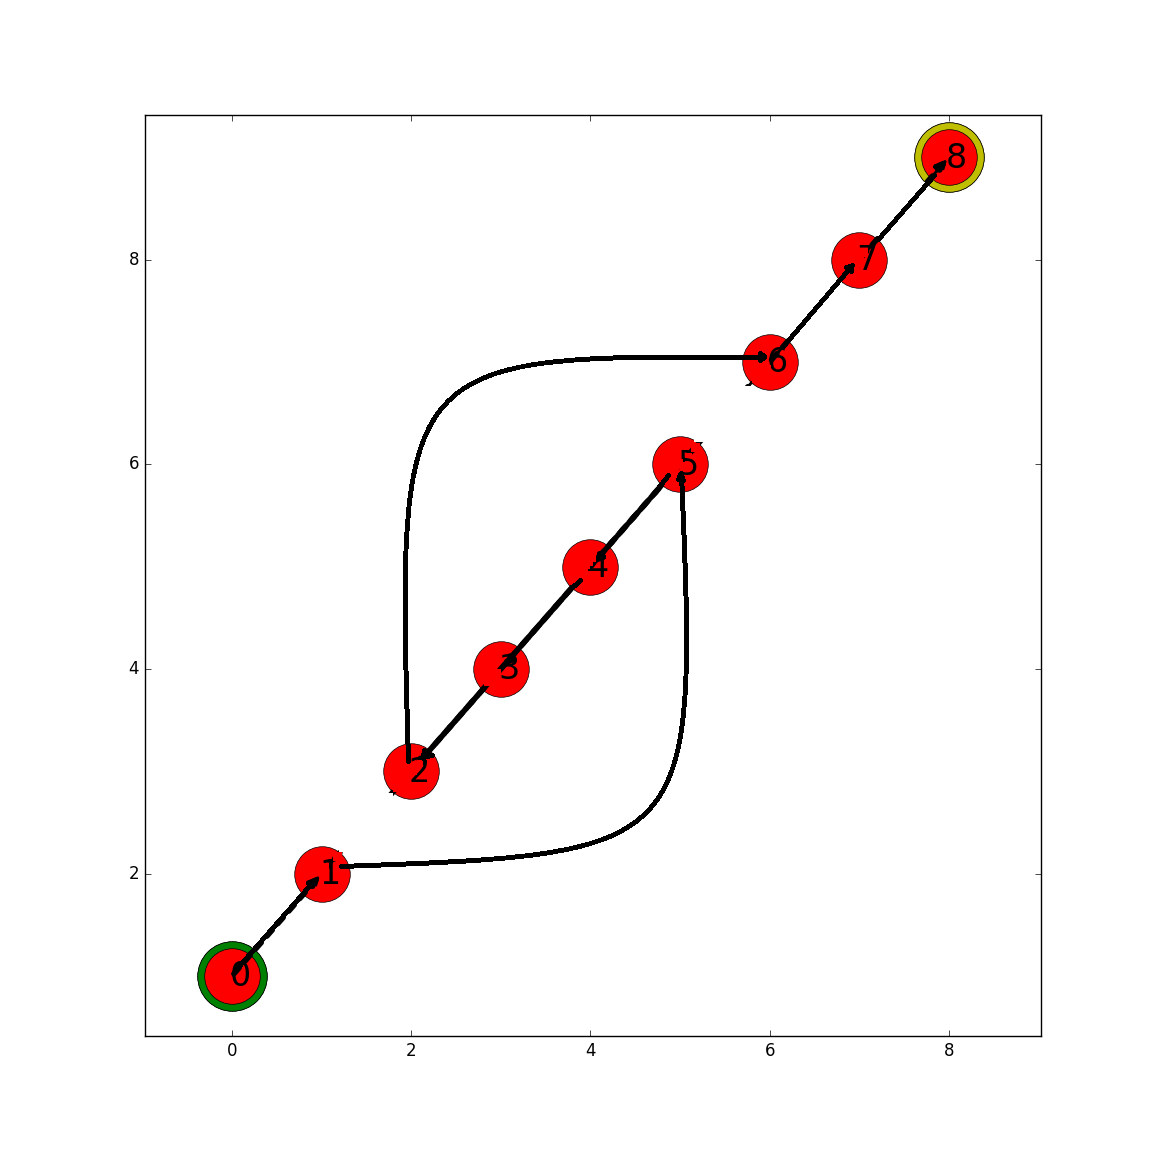
\includegraphics[scale=0.3]{./EJ3/ejemplo2opt.png}\\
 {            \textit{Movimiento 2-opt}}
  \end{center}
  \vspace*{0.3cm}

Realizar un movimiento $2-opt$ como se explicó, es cambiar dos aristas de un recorrido por otras dos aristas diferentes, de manera tal que el resultado siga siendo un recorrido simple.
En el ejemplo puede observarse el recorrido 1->2,3,4,5->6,7,8 y el movimiento realizado cambia las aristas (1,2) y (5,6) por las aristas (2,6) y (1,5), lo que invierte el tramo 2,3,4,5 a 5,4,3,2 obteniendo el recorrido 1,5,4,3,2,6,7,8.
  
  \vspace*{0.3cm} \vspace*{0.3cm}
  \begin{center}
 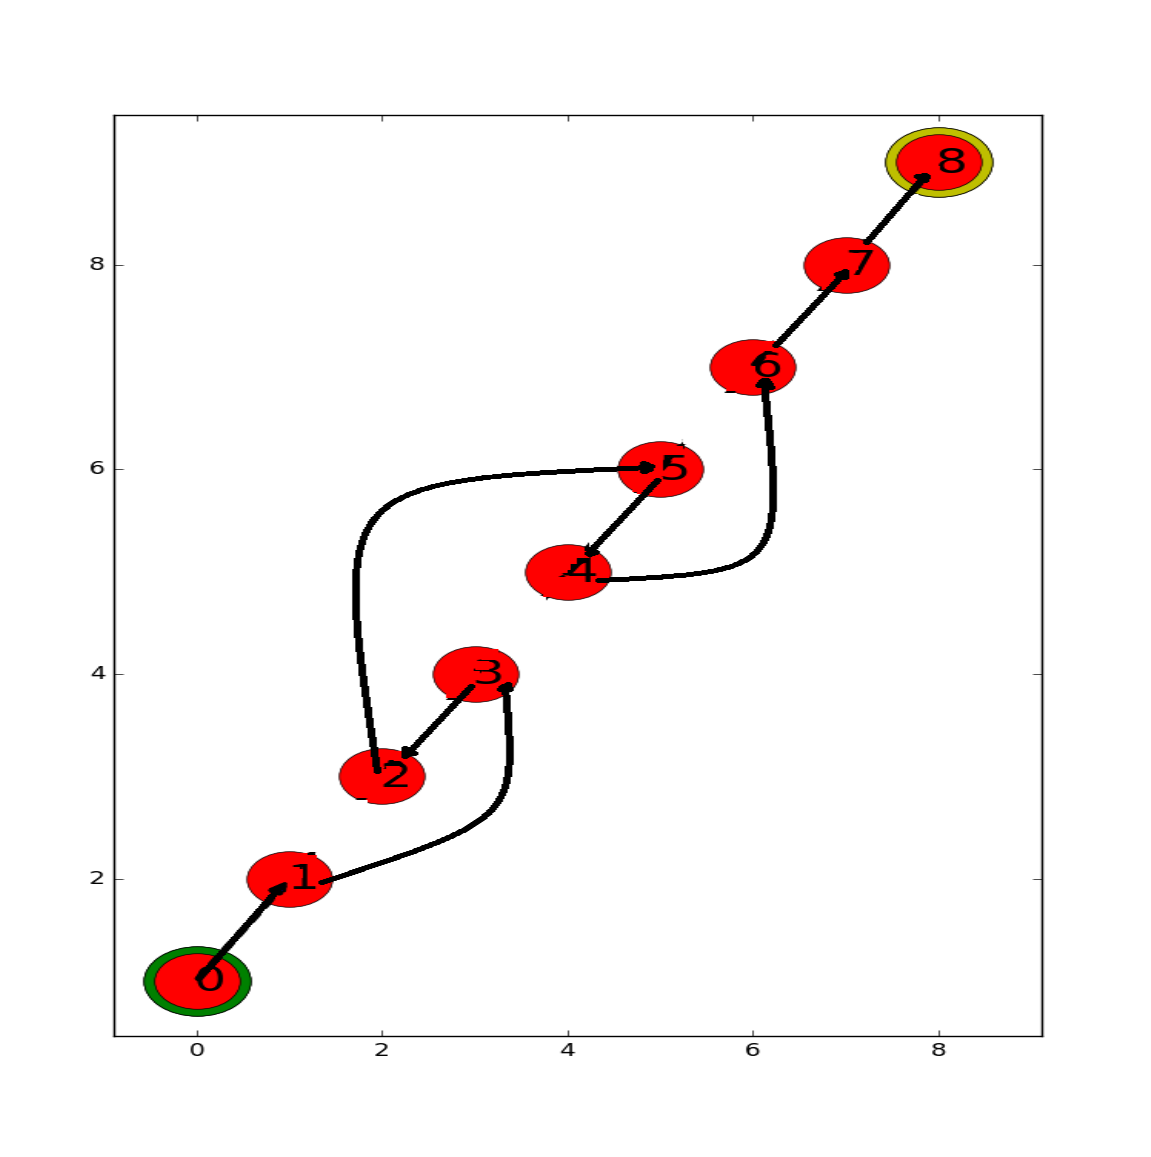
\includegraphics[scale=0.3]{./EJ3/ejemplo3optCaso1.png}\\
 {            \textit{Movimiento 3-opt}}
  \end{center}
  \vspace*{0.3cm}
  
Realizar un movimiento $3-opt$ genera más de una opción para las tres aristas elegidas.
En el ejemplo podemos ver el recorrido 1->2,3->4,5->6,7,8 y se eligen las aristas (1,2), (3,4) y (5,6) intercambiandolas por (1,3), (2,5) y (4,6) y obteniendo el recorrido 1->3,2->5,4->6,7,8.

Aunque existen otras seis posibilidades, tres más son $3-opt$ y otras tres que incluyen dos movimientos $2-opt$ cada una. Si lo que se busca es $3-opt$ puro, deben descartarse las que sean $2-opt$.

Los movimientos $3-opt$ restantes serán:

\begin{enumerate}
\item 1->4,5->2,3->6,7,8
\item 1->5,4->2,3->6,7,8
\item 1->4,5->3,2->6,7,8
\end{enumerate}

$3-opt$ requerirá que se tomen todas estas posibilidades si se busca no dejar ningún caso afuera.

Además, realizando un simple swap de nodos, podemos obtener muy fácilmente soluciones que intercambian 2 o 4 aristas. Serán dos si los nodos intercambiados de posición son consecutivos y cuatro si no lo son.

\vspace*{0.3cm} \vspace*{0.3cm}
  \begin{center}
 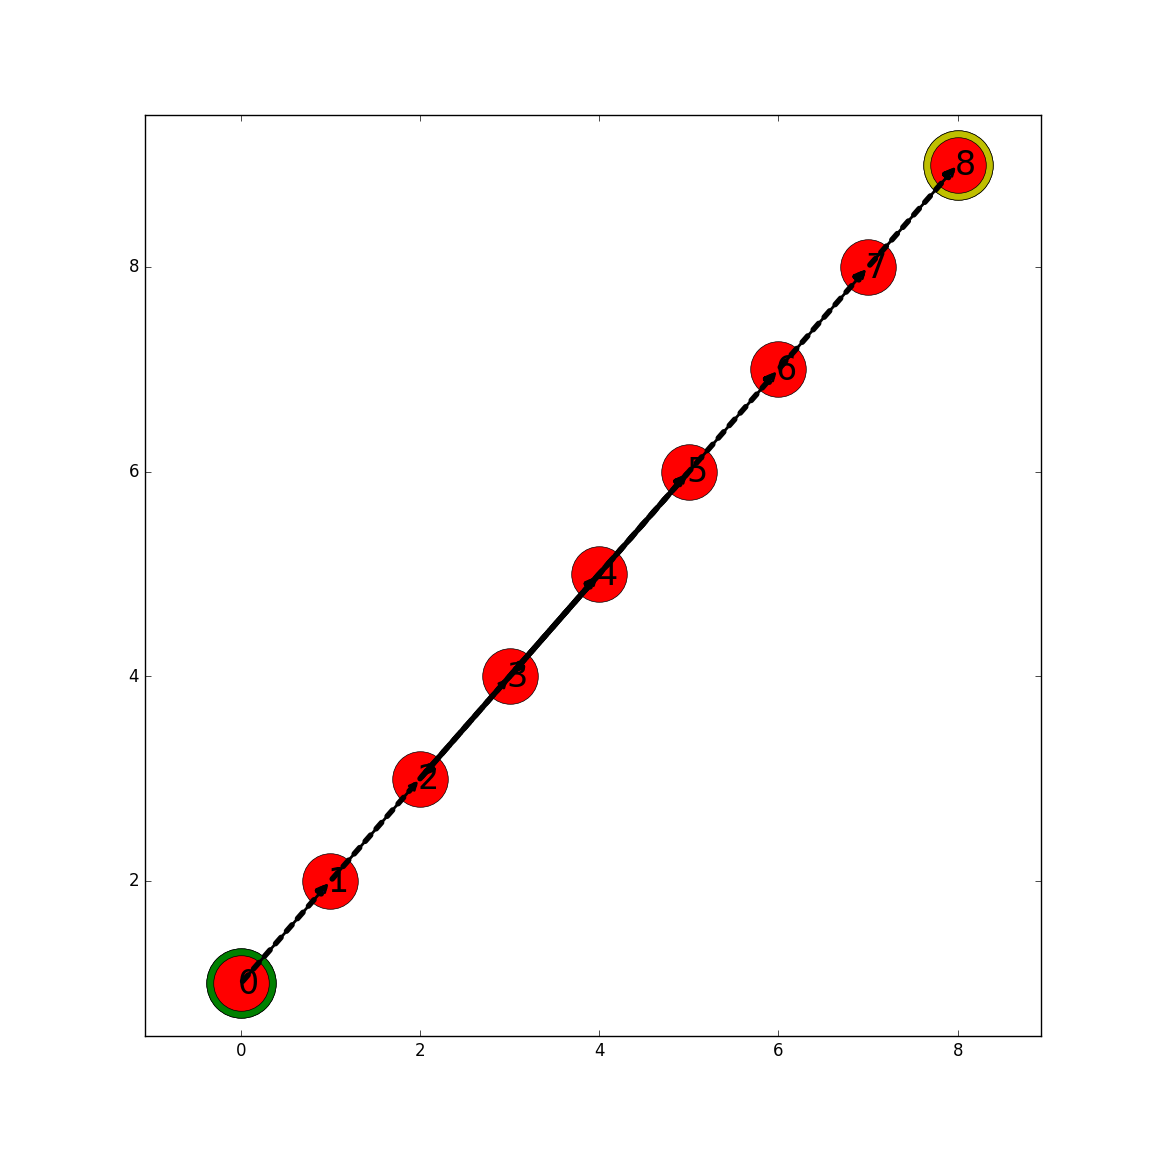
\includegraphics[scale=0.3]{./EJ3/ejemploSwap.png}\\
 {            \textit{Movimiento swap}}
  \end{center}
  \vspace*{0.3cm}

En el ejemplo se toma el camino 1,2,3,4,5,6,7,8 y se intercambian 2 por 6 generando 1,6,3,4,5,2,7,8 y generando asi 4 aristas nuevas (1,6), (6,3), (5,2) y (2,7).

Además tenemos que tener en cuenta para nuestro problema, que al permutar una solución con alguno de los métodos mencionados, y la solución sea válida, pueden quedar pokeparadas al final del recorrido, por lo cual es necesario eliminarlas del mismo, ya que al considerar el recorrido hasta las mismas, se podría sumar distancia a la solución que ya no aporta, debido a que todos los gimnasios fueron derrotados. Además, podría desestimarse como solución candidata si luego se obtiene otra que tiene menor distancia solo porque se están contando pokeparadas de más.\\

De esta manera, podremos movernos a través del espacio de soluciones locales a $S_o$ y tal vez mejorar la solución, aunque que de esto, por ser una heurística, no tendremos ninguna garantía.

En este punto nos centraremos en estudiar y tratar de concluir cual de las heurísticas consideradas en este punto es mejor utilizar para mejorar los resultados obtenidos por el algoritmo goloso del punto anterior. Es decir, dado un tipo de entrada, que en este caso se corresponde con un mapa de pokeparadas y gimnasios, que tendrá alguna particularidad que hará que el algoritmo goloso produzca un resultado bueno o malo, veremos que tipo de busqueda local será mejor aplicar para mejorar la solución o si no conviene aplicar ninguna de las heurísticas de este punto ya que a pesar de ser la solución buena o mala, no se obtienen mejores resultados.

Primero veremos los pseudocódigos de las tres heurísticas y analizaremos sus complejidades. Luego realizaremos un análisis cualitativo de las mismas aplicadas a los resultados de cada tipo de entrada, tratando de abordar las características de las mismas y explicar porque una heurística resulta mejor o no en cada caso. Luego de comparar los resultados para cada tipo de entrada intentaremos elegir, si es posible, el tipo de búsqueda local que obtiene los mejores resultados en la mayoría de los casos.

%y si es posible haremos un análisis para determinar si podría haberse obtenido una solución mejor intercambiando más aristas.
